\section{Cartes}

\subsection{Carte IHM}
\begin{frame}
    \frametitle{Carte IHM}
    La carte IHM (Interface Homme-Machine) va nous permettre de sélectionner grâce aux boutons poussoirs de sélectionner le programme désiré. Les LEDs s'allumeront ensuite pour prévenir que le programme est lancé.

    \vfill
    \begin{figure}[H]
        \centering
        \begin{minipage}{.5\textwidth}
            \centering
            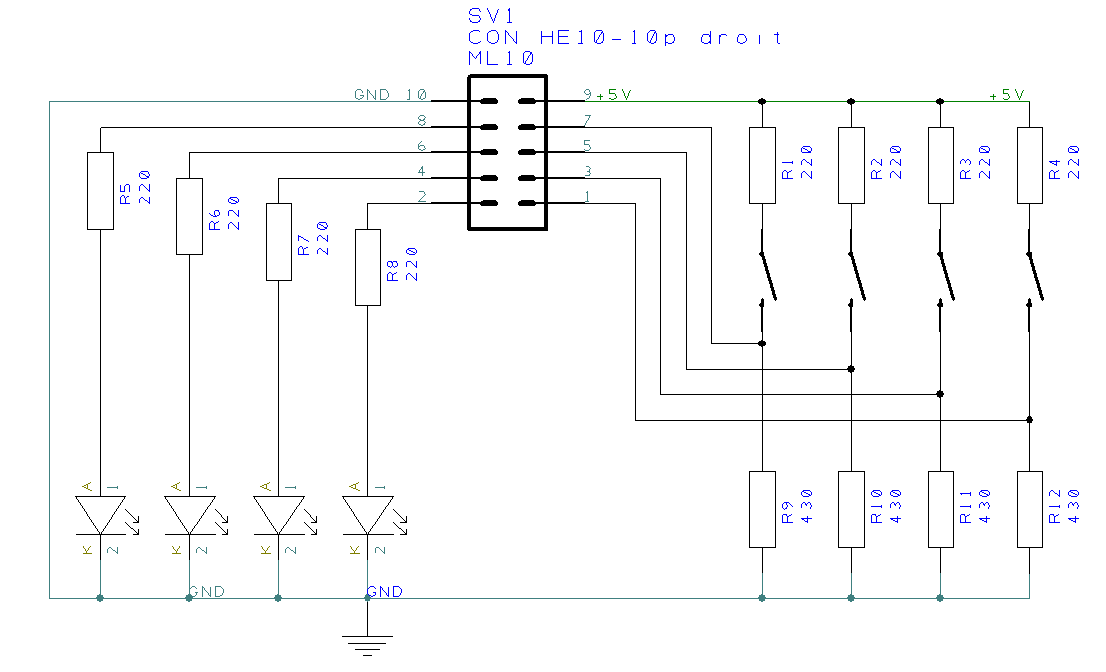
\includegraphics[width=.7\linewidth]{Images/carteIHM_sch.png}
            \caption{Carte IHM - Schématic}
            \label{fig:ihmsch}
        \end{minipage}%
        \begin{minipage}{.5\textwidth}
            \centering
            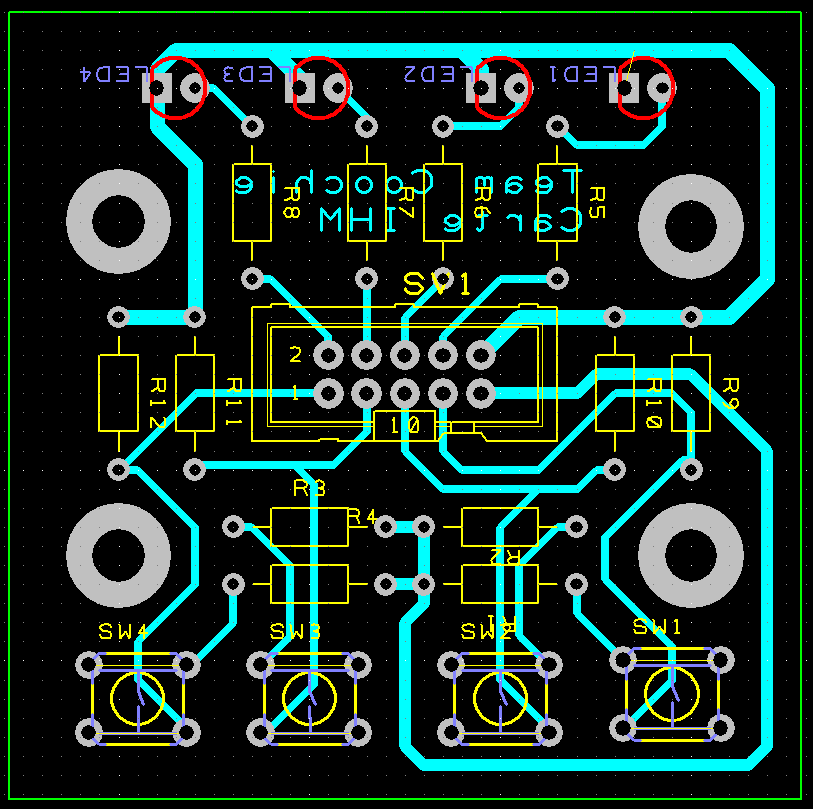
\includegraphics[width=.5\linewidth]{Images/carteIHM_pcb.png}
            \caption{Carte IHM - PCB}
        \label{fig:ihmpcb}
        \end{minipage}
    \end{figure}
    
\end{frame}

\subsection{Carte Capteurs}
\begin{frame}
    \frametitle{Carte Capteurs}
    La carte capteurs est équipée de quatre capteurs TCRT5000 et va permettre au robot de s'orienter dans l'espace et de s'adapter aux contraintes imposées (ligne blanche, confettis, ...).

    \vfill
    \begin{figure}[H]
        \centering
        \begin{minipage}{.5\textwidth}
            \centering
            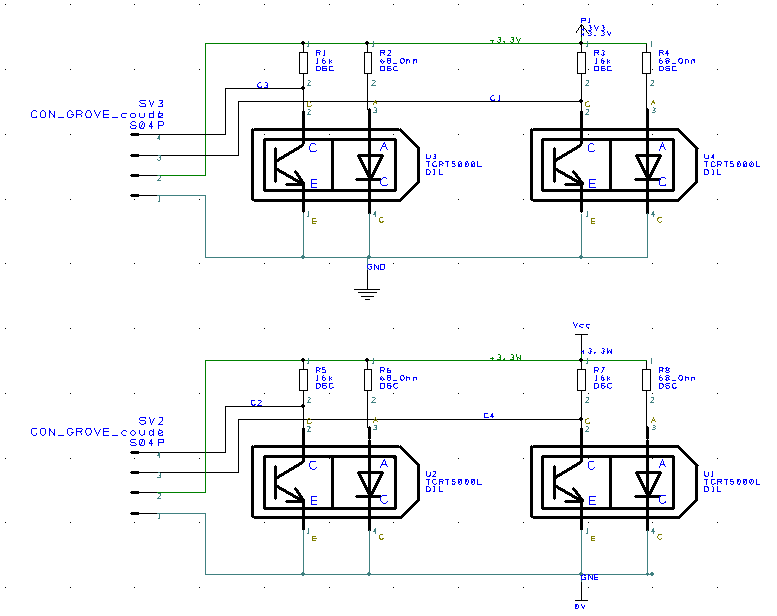
\includegraphics[width=.7\linewidth]{Images/carteCapteurs_sch.png}
            \caption{Carte Capteurs - Schématic}
            \label{fig:ihmsch}
        \end{minipage}%
        \begin{minipage}{.5\textwidth}
            \centering
            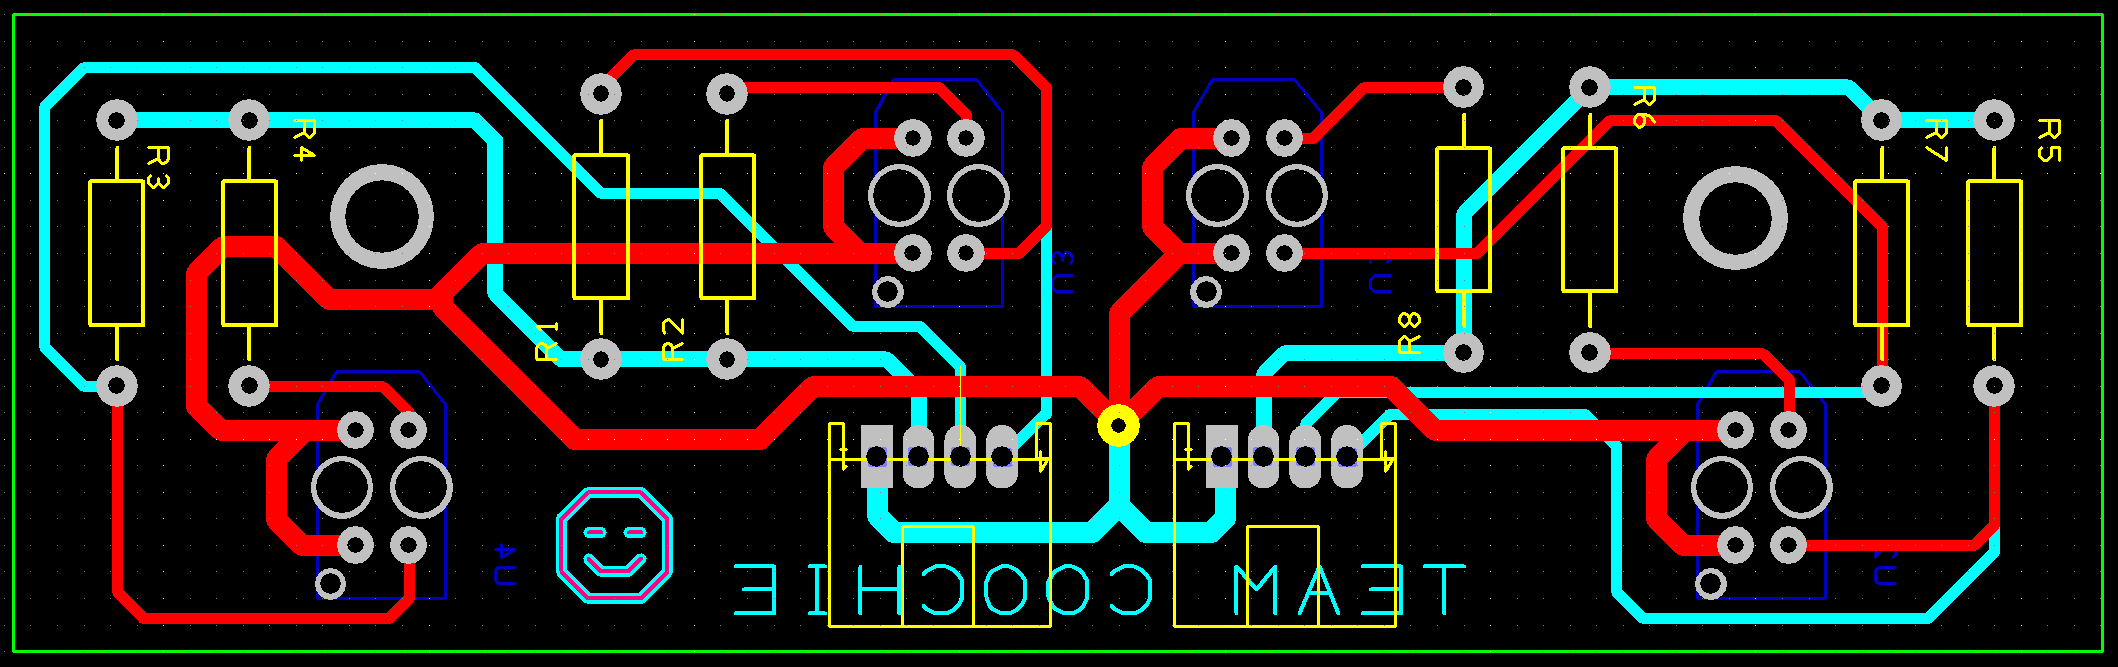
\includegraphics[width=.5\linewidth]{Images/carteCapteurs_pcb.png}
            \caption{Carte Capteurs - PCB}
        \label{fig:ihmpcb}
        \end{minipage}
    \end{figure}
\end{frame}

\subsection{Carte Hacheur}

\subsection{Carte Commande}
    \begin{frame}
    \frametitle{Carte Commande}
    \framesubtitle{SAE Robot - Team Coochie}
    \begin{itemize}
        \item A typical slide has bulleted lists
        \item These can be uncovered in sequence
    \end{itemize}
\end{frame}